\chapter{Domain Analysis}
Given the complexity of the domain, it was decided to use Event Storming to become familiar with the terminologies and workflows typical of the domain. The adoption of this activity was also justified by having real domain experts available to explain to us the current business processes. In addition, using this approach it was possible to bring together managers from different areas, who collaborated to correctly define the dynamics and problems concerning their communication.

\section{Subdomains}
These are the subdomains that emerged from the Event Storming process:
\begin{itemize}
    \item Production Planning: creates the daily production planning
    \item Milk Planning: estimates the amount of milk to order each week
    \item Stocking: manages the packaging of cheeses and their stocking
    \item Restocking: orders the milk and keeps track of the available quantity of milk
    \item Client Orders: handles and fulfills the orders made by clients
    \item Production: tracks the cheeses' production process
    \item Pricing: calculates the price for every order considering the specific client
\end{itemize}

We proceeded with this exploration of the domain by individuating the subdomains where digital twins would have been crucial to help the processes.
The two subdomains we selected were \textit{Milk Planning} and \textit{Stocking} \ref{img:event-storming}.
The decision was made considering the added value that the digital twins could bring to the processes (this aspect will be explored in the\ref{sec:dt-motivations} section) and the fact that the two subdomains were quite complex.
The \textit{Stocking} subdomain is the one that manages the quality assurance of the cheeses, which is a crucial process for the company.
The \textit{Milk Planning} subdomain is the one that estimates the amount of milk to order each week, which is a process that is very important for the company's financial health.

\begin{figure}[H]
    \centering
    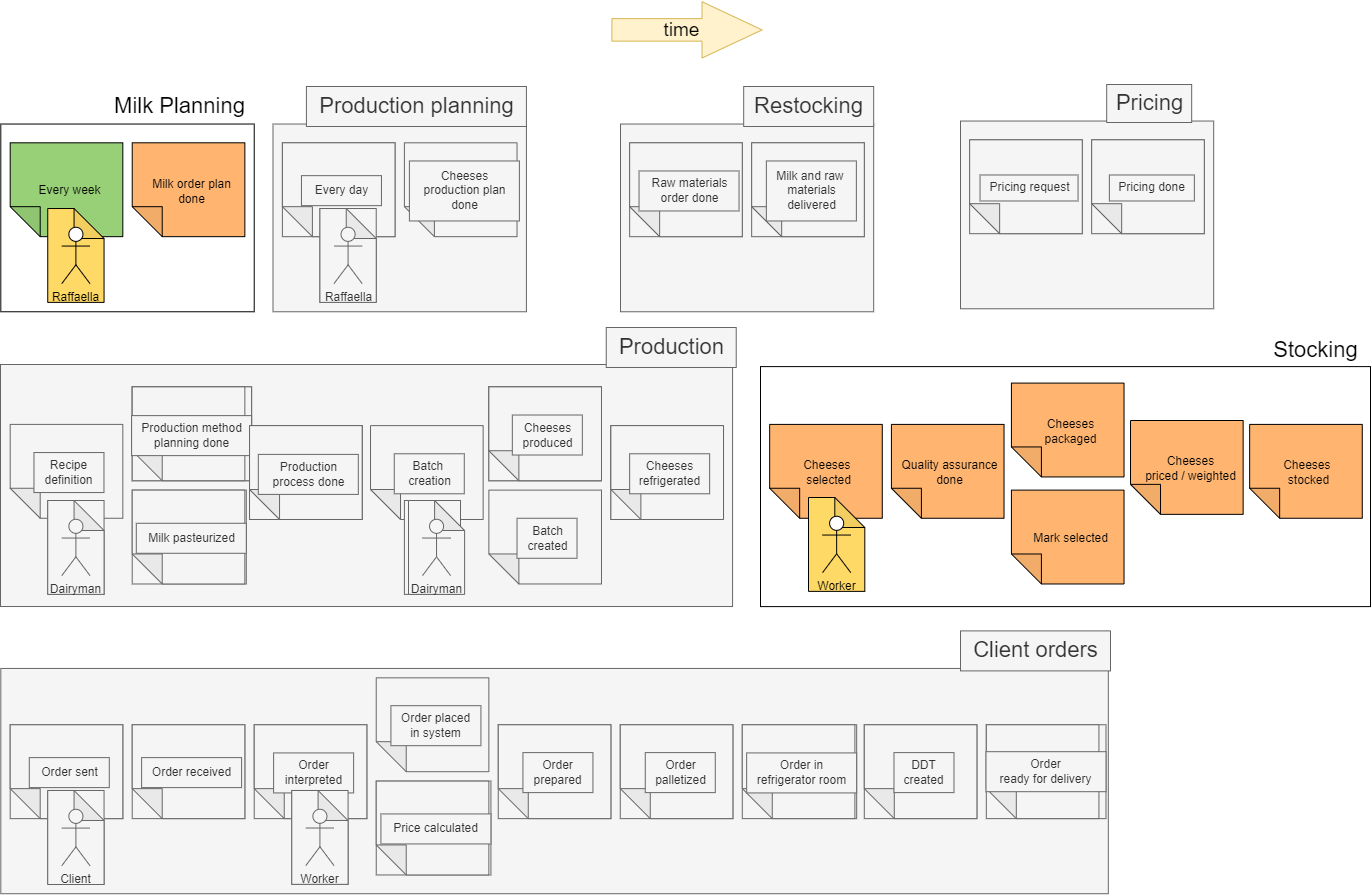
\includegraphics[width=\textwidth]{img/event-storming.png}
    \caption{Event storming result. The image highlights the two subdomains we selected for interacting with the digital twins}
    \label{img:event-storming}
\end{figure}

\section{Digital Twins - motivations}\label{sec:dt-motivations}
This section will describe the digital twins that were chosen to be implemented in the project and the motivations behind the choice of inserting them in this context.

\subsection{Milk Tank Digital Twin}
Milk storage is a crucial aspect for several reasons: milk yield, product quality, and parameters to be met.

At present, milk storage management is done manually: once stored, the milk lies until a new production is required.
Before production begins, an analysis is conducted on the milk to detect its pH, protein level and other parameters.
In addition to being a cost to the farm, this operation represents a loss of time in cheese production: it takes an operator about thirty minutes to
perform this kind of analysis.
Another factor that can affect the quality of milk is temperature changes: continuous temperature changes can alter the structure of milk and be 
reflected in a lower yield during processing or even in non-use.
Finally, the integration of milk tanks with the farm information system is absent, so there is no information about the status of stored milk.
Integration with the cheese processing machinery is partial; in fact, it is an operator who has to issue the start processing command to open the 
tank valve and then proceed with processing.

To solve most of the raised weaknesses, we believe that the use of digital twins for the milk tank can be an effective tool.
In fact, with the use of a digital twin, we can guarantee real-time monitoring of the milk and intelligently control the milk parameters for 
production.
Modeling the milk tank with a digital twin leads to the advantage of always having the latest information about the quantity of milk stored,
which is useful both for planning the reordering of milk and for the production management system.
Even if there must be a temporary disruption such that the tank no longer communicates with the rest of the system,
the latest information on the quantity of milk stored is still available in the twin.
In this way, we ensure that some of the services continue to work even in the event of temporary failures.

Finally, it is useful to have early warnings in case critical situations occur, such as a pH value that is too high (or too low), or fluctuations in
temperature.
In this regard, provision has been made for the digital twin to propagate messages so that timely action can be taken.

The use of a digital twin in this scenario is advantageous for several reasons: human intervention to perform milk analysis is minimized as there is
real-time monitoring of all key parameters, thus reducing the time to go into production.
As a consequence of real-time analysis, there is a guarantee that the milk used reflects all requirements thus maximizing product quality and yield.
Also as a consequence of the real-time analysis of all parameters, an alarm system is available to enable timely action to avoid waste and loss of time.

\subsection{Packaging Machine Digital Twin}
During meetings with domain experts, it emerged that the packaging of products is done by automatic machines that pack the cheeses.
These machines are set up by an operator, and it is not uncommon for mistakes to be made in the setup, which can cause damage to the product or even
the machine. It has been reported to us that these kinds of machines often break down causing a delay in the packaging line.

Following on from the considerations made earlier, it was studied how through digital twins it is possible to minimize errors made by humans and
predict breakdowns from machines to intervene promptly and eliminate dead time due to extraordinary machine maintenance.

To solve the problem of human error, we modeled the digital twin so that the system in charge of handling packaged products can interact and set the
batch to be packaged.
In this way, we eliminate the human component by reducing the errors that can be made.
In addition, we can automate the entire process of machine setup, an operation that is currently done by an operator on the machine.

The aspect of reducing time due to maintenance is a crucial aspect that digital twins can solve~\cite{doi:10.1080/0951192X.2019.1686173}.
Through machine learning techniques and leveraging digital twins, the RUL of the machinery can be determined, all corroborated by simulations that
signal any impending breakdowns.

\subsection{Scale Digital Twin}
Just as with the metal detector, the scale is also subject to stringent regulations. The measurement of product weight must meet legal parameters
outside of which the product cannot be sold.
A weight below the declared weight would represent fraud against the consumer; conversely, a weight above the declared weight represents a loss for the company.
The scale could be used to monitor the weight of the packages and detect if there are any anomalies. If so, it may be a sign of a problem in the packaging process (e.g. deformed molds).

Domain experts explained to us that scales can provide reports but these are not integrated with the business information system. Again, digital 
twins can help integrate such data into the system and interact with the system for storage going in a direction of total automation of the packaging
line.

\subsection{Metal detector Digital Twin}
A metal detector is an indispensable tool in the quality assurance process, stringent regulations require its use within the packaging line.
In one of the meetings with domain experts, it emerged that the metal detector is almost isolated in terms of communication with other devices, and
the data it produces is not integrated into the company's information system.

The detection of metallic components is, however, very rare and could imply that the machine to make cheese might have deteriorated. So, along with checking the batch where the anomaly is detected, a check of the machine could also be performed.

With the use of a digital twin we want on the one hand to better integrate the data that the machinery can produce and on the other hand we
want it to be able to easily communicate with other machinery in the line.

\section{Supporting bounded contexts}
Having introduced digital twins we noticed that other subdomains or bounded contexts were needed in order to support their functioning.
In particular, we identified the following bounded contexts:
\begin{itemize}
    \item Alerts: manages the alerts sent by the digital twins
    \item Maintenance: manages the maintenance of the Packaging Machine digital twin
    \item Reporting: manages the reports sent by the Scale and the Metal Detector digital twins
\end{itemize}

The \textit{Alerts} bounded context is responsible for collecting the fault messages coming from the digital twins, storing them and notifying the responsible people.

For instance, \textit{Milk Tank} would notify any anomaly in the milk quality (pH or temperature values out of range);
\textit{Packaging Machine} would notify any anomaly in the machine status (e.g. a broken part) and \textit{Scale} and \textit{Metal Detector} would notify any anomaly in the weight or the presence of metal.

The \textit{Maintenance} bounded context was mainly introduced to predict the maintenance of the Packaging Machine digital twin but its use could be extended to other machines.

Finally, the \textit{Reporting} bounded context was introduced to collect the reports sent by the Scale and the Metal Detector digital twins and to do some basic analysis on this data.
Given its simplicity and the fact that it doesn't add business differentiation, this bounded context will be outsourced to a third-party company.

The figure\ref{img:subdomains-dt} shows the bounded contexts and the digital twins that interact with them.

\begin{figure}[H]
    \centering
    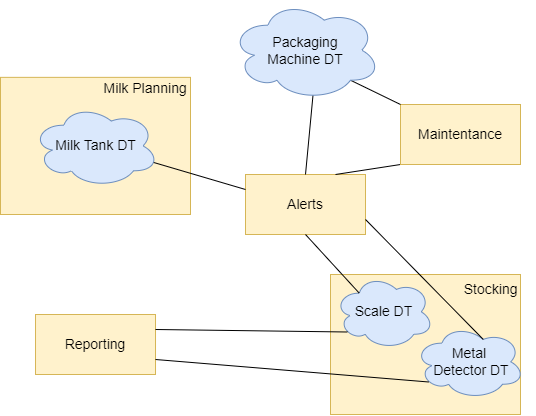
\includegraphics[width=0.8\textwidth]{img/subdomains-dt.png}
    \caption{The supporting bounded contexts and their interactions with the digital twins}
    \label{img:subdomains-dt}
\end{figure}

\section{Business differentiation}
We then proceeded to have a more in-depth analysis of each subdomain to determine their business differentiation and to do a first estimate of the model's complexity. The following considerations were made:
\begin{itemize}
    \item Production Planning and Milk Planning are to be considered core subdomains since they can be decisive in order to optimize the efficiency of the factory
    \item the Milk Planning subdomain can be seen as a big-bet subdomain since it has the potential to significantly disrupt the market if implemented in such a way that can predict trends and spikes in orders
    \item the Reporting subdomain is considered as outsourced since it is not a core subdomain and it is not a big-bet subdomain either. It is also not a subdomain that can be considered a differentiator for the company.
    \item the remaining subdomains introduce a lower amount of business differentiation, so they are to be considered as supporting subdomains
\end{itemize}

We gathered these pieces of information and compiled the following core domain chart:

\begin{figure}[H]
    \centering
    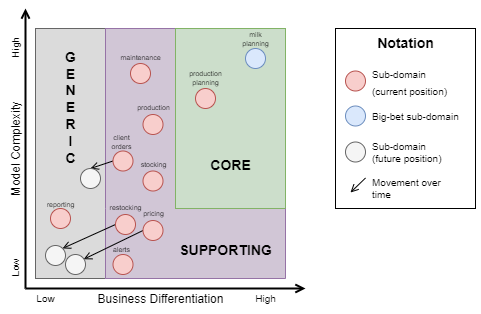
\includegraphics[width=\textwidth]{img/core-domain-chart.png}
    \caption{The core domain chart of the identified subdomains}
    \label{img:core-domain-chart}
\end{figure}
